    \documentclass[conference]{IEEEtran}
    \IEEEoverridecommandlockouts
    % The preceding line is only needed to identify funding in the first footnote. If that is unneeded, please comment it out.


    \usepackage{cite}
    \usepackage{amsmath,amssymb,amsfonts}
    \usepackage{algorithmic}
    \usepackage{algorithm}
    \usepackage{float}
    \usepackage{graphicx}
    \usepackage{textcomp}
    \usepackage{xcolor}
    \usepackage{url}
    \usepackage{array}        % for m{} and \newcolumntype
    \usepackage{longtable}    % multipage tables
    \usepackage{booktabs}     % optional: nicer rules (not used below but useful)
    % define a reusable centered-and-vertically-centered column type
    \newcolumntype{M}[1]{>{\centering\arraybackslash}m{#1}}
    % spacing tweaks (optional)
    \setlength{\extrarowheight}{2pt}
    \setlength{\tabcolsep}{6pt}

    \begin{document}

    \title{\textbf{A Survey \& Research Gap Analysis: \\
    Integrating AI and Barcode Scanning for Ingredient Analysis and Personalized Health}}

    \author
    {\IEEEauthorblockN{1\textsuperscript{st} Harshal Unde}
    \IEEEauthorblockA{\textit{Department of Computer Engineering} \\
    \textit{Ramrao Adik Institute of Technology}\\
    D. Y. Patil Deemed to be University\\ 
    Navi Mumbai, India\\
    harshal.unde@rait.ac.in}
    \and
    \IEEEauthorblockN{2\textsuperscript{nd} Vanita Mane}
    \IEEEauthorblockA{\textit{Department of Computer Engineering} \\
    \textit{Ramrao Adik Institute of Technology}\\
    D. Y. Patil Deemed to be University\\ 
    Navi Mumbai, India\\
    vanita.mane@rait.ac.in}
    \and
    \IEEEauthorblockN{3\textsuperscript{rd} Tushar Ghorpade}
    \IEEEauthorblockA{\textit{Department of Computer Engineering} \\
    \textit{Ramrao Adik Institute of Technology}\\
    D. Y. Patil Deemed to be University\\ 
    Navi Mumbai, India\\
    tushar.ghorpade@rait.ac.in}
    }

    \maketitle

    \begin{abstract}
    The increasing consumption of packaged foods and the rising incidence of lifestyle-related disorders such as diabetes, hypertension, obesity, and food allergies have created a need for intelligent tools that can interpret food labels and provide personalized dietary guidance. Existing food analysis applications typically rely on either barcode-based product lookup or optical character recognition (OCR) of packaging text, each with inherent limitations including incomplete database coverage, sensitivity to label variability, and lack of comprehensive personalization. This paper presents a fully implemented Artificial Intelligence–driven system that integrates barcode scanning, OCR-based ingredient extraction, and user-specific health profiling to deliver real-time ingredient safety analysis and personalized nutritional assessment.

    The proposed system uses a hybrid data ingestion pipeline capable of processing both structured product data and unstructured label images. When barcode information is unavailable or insufficient, the OCR module extracts ingredient and nutritional details directly from packaging. A knowledge-driven ingredient safety engine evaluates these components against a curated database of allergens, additives, and condition-specific risk factors. The system further incorporates detailed user profiles—including medical conditions, allergies, and dietary preferences—to generate context-aware recommendations. A macronutrient analysis module assesses key nutritional parameters relative to recommended intake levels, while a personalized verdict module produces clear guidance such as “Safe,” “Caution,” or “Avoid,” along with explanatory feedback.

    Designed for real-time use and broad market applicability, the hybrid framework improves coverage, interpretability, and decision relevance compared to single-method solutions. The system demonstrates how multimodal analysis combined with personalized health awareness can support informed consumer choices and contribute to digital health empowerment.
    \\

    \textbf{Keywords}: Artificial Intelligence, Food Label Analysis, Ingredient Safety Assessment, Optical Character Recognition, Barcode Scanning, Personalized Nutrition, Allergen Detection, Packaged Food Evaluation.
    \end{abstract}

\section{Introduction}

The rapid evolution of dietary patterns driven by urbanization, globalization of food markets, and the widespread availability of ultra-processed packaged products has substantially increased dependence on front-of-pack nutritional information for everyday purchasing decisions. In developing economies such as India, where consumption of packaged foods has risen sharply, consumers routinely encounter complex ingredient lists, additives, preservatives, and detailed nutrient disclosures that are difficult to interpret without specialized knowledge. Regulatory bodies such as the Food Safety and Standards Authority of India (FSSAI) have introduced labeling standards, QR-code initiatives, and compliance frameworks to enhance transparency. However, the effectiveness of these measures largely depends on consumers’ ability to understand and contextualize the provided information [16]. Research indicates that limited nutrition literacy, combined with time pressure during shopping, often prevents meaningful interpretation—particularly for individuals managing chronic diseases [13], [14].

At the same time, the global prevalence of non-communicable diseases—including diabetes, hypertension, cardiovascular disorders, obesity, and food allergies—continues to escalate, creating an urgent demand for tools that enable informed dietary decisions in real time. Mobile health technologies and intelligent decision-support systems have demonstrated significant potential in assisting disease management and encouraging healthier consumption behaviors [13], [17]. Nevertheless, many existing applications require manual food logging, depend on static databases, or provide generalized advice that does not account for individual physiological variability or multiple coexisting medical conditions [21], [29]. This mismatch between available nutritional information and actionable personalized guidance remains a major obstacle to effective digital health interventions.

Barcode-based food scanning applications represent one of the earliest and most widely adopted solutions for automated product identification. Platforms such as FoodSwitch and Nutrilens illustrate how standardized product identifiers can be decoded to retrieve nutritional data from centralized repositories [2], [15]. These approaches are computationally efficient and well suited for real-time deployment on mobile devices. However, their performance is highly dependent on database completeness, accuracy, and regional coverage. Newly introduced products, locally manufactured items, or poorly cataloged goods may not be recognized, resulting in incomplete information and reduced reliability [2], [10].

To address these shortcomings, researchers have explored optical character recognition (OCR) and computer vision techniques that extract ingredient lists and nutritional values directly from packaging images. Systems such as NutriScan and segmentation-based models like IngredSAM demonstrate significant progress in automated label interpretation [1], [6]. Such methods extend applicability to products absent from databases and to diverse packaging formats, but they introduce challenges related to image quality, multilingual text, layout variability, and processing overhead [23], [28]. Additionally, OCR-based approaches often operate independently of regulatory datasets, limiting their ability to verify authenticity or standardized nutrient values [16].

Another important research direction focuses on personalized nutrition and health-aware recommendation systems. Advanced artificial intelligence models can generate dietary guidance tailored to individual health profiles, disease conditions, and lifestyle factors [8], [9], [26]. Clinical and mobile health studies indicate that personalized recommendations can improve disease outcomes and support long-term behavioral change [13], [14], [17]. Despite these advances, most personalization frameworks rely on manually entered dietary logs or structured datasets rather than real-time evaluation of packaged foods. As a result, a significant gap persists between product recognition technologies and individualized health assessment.

Comprehensive reviews suggest that many existing solutions address only a single component of the broader problem—either product identification, ingredient interpretation, or personalized recommendation—leading to fragmented systems with limited real-world effectiveness [19], [21]. Hybrid approaches combining barcode scanning with image-based analysis have been proposed to improve coverage, as demonstrated by applications such as Allertify and Nutriknow [3], [4]. However, these systems are typically designed for narrow objectives, such as allergen detection, and often lack comprehensive health profiling, regulatory integration, or adaptive decision mechanisms. Moreover, most assume a static health profile and do not consider multiple simultaneous conditions, medication interactions, or temporary physiological changes that can influence dietary suitability [18], [20].

A preliminary survey conducted for this study identified three major unresolved challenges:
(1) the absence of tightly integrated hybrid scanning frameworks that intelligently combine barcode and OCR modalities;
(2) insufficient support for comprehensive personalization across multiple health conditions; and
(3) the lack of mechanisms for dynamic, context-aware interpretation of nutritional data.
Addressing these issues requires a unified architecture capable of integrating structured regulatory information, unstructured visual data, and individualized health context within a single decision pipeline.

In response, this paper presents a fully implemented Artificial Intelligence–driven system for ingredient analysis and personalized health assessment of packaged foods. The proposed solution integrates barcode scanning, OCR-based text extraction, knowledge-driven ingredient safety evaluation, macronutrient analysis, and user-specific health profiling to produce interpretable recommendations at the point of consumption. Unlike existing modular tools, the framework employs a hybrid data ingestion strategy that prioritizes verified product metadata when available while seamlessly switching to image-based analysis for unregistered items. It also incorporates a rule-guided personalization engine capable of evaluating multiple chronic conditions, allergies, dietary preferences, and contextual health factors simultaneously.

The primary contributions of this work are summarized as follows:

\begin{itemize}
    \item A unified hybrid architecture that combines barcode retrieval and OCR-based label understanding within a single operational workflow.
    \item A comprehensive ingredient safety engine built on a curated knowledge base of allergens, additives, and condition-specific risk factors.
    \item A personalized verdict generation mechanism that converts complex nutritional data into clear, actionable guidance tailored to individual health profiles.
    \item A deployable real-time system designed for scalability, usability, and applicability across diverse packaged food environments.
\end{itemize}

By bridging the gap between automated product recognition and personalized digital health support, the proposed framework aims to empower consumers with accurate, context-aware dietary insights and advance the development of intelligent food analysis platforms. The remainder of this paper presents the related work, system architecture, methodology, evaluation results, and directions for future research.

\section{Related Work}

The rapid advancement of intelligent packaged food analysis systems is closely linked to developments in mobile computing, computer vision, and artificial intelligence. Increasing public awareness of nutrition, the growing burden of lifestyle-related diseases, and regulatory efforts to improve labeling transparency have collectively encouraged research into automated interpretation of food labels and personalized dietary assistance. Existing studies can generally be grouped into four interconnected areas: barcode-based food scanning tools, AI-driven ingredient recognition techniques, personalized health recommendation systems, and quantitative frameworks for nutritional evaluation. This section reviews prior work across these domains, highlighting their contributions and limitations while establishing the context for the proposed hybrid approach.

\subsection{Barcode-Based Food Scanning Applications}

Barcode scanning is one of the earliest and most widely adopted methods for evaluating packaged foods through mobile applications. These systems decode standardized identifiers—such as UPC or EAN codes—and retrieve corresponding product information from centralized databases, including nutritional values, ingredient lists, and manufacturer details. Applications like FoodSwitch and Nutrilens demonstrate that barcode-based lookup can provide rapid access to structured product data with minimal computational requirements and high accuracy for registered items [2], [15].

Several investigations indicate that such tools can positively influence consumer purchasing behavior by increasing awareness of nutritional attributes such as sugar, salt, and fat content [10], [11]. Because barcode decoding is computationally lightweight, these applications are suitable for real-time deployment on smartphones and function effectively even in low-resource environments. Large backend databases also enable aggregation of product-level insights across regions.

Despite these advantages, barcode-based systems are fundamentally limited by the completeness and timeliness of their databases. Newly introduced products, region-specific brands, locally produced items, or incorrectly cataloged goods may lack associated metadata, resulting in incomplete analysis or recognition failure [2], [10]. Moreover, barcode lookup typically provides product-level summaries rather than detailed ingredient interpretation, reducing usefulness for individuals with allergies, dietary restrictions, or medical conditions. Most implementations also deliver generalized nutritional feedback without incorporating personalized health context.

Efforts to enhance barcode systems through QR-code labeling and traceability mechanisms have been explored to provide richer product information and supply-chain transparency [5]. However, inconsistent standards and limited industry adoption have hindered widespread effectiveness. Consequently, barcode-based methods alone cannot ensure comprehensive coverage of diverse food markets.

\subsection{AI-Powered Ingredient Recognition Systems}

To address the dependency on preexisting databases, researchers have increasingly explored AI-driven techniques that extract information directly from packaging. Optical Character Recognition (OCR), computer vision, and natural language processing allow systems to interpret ingredient lists and nutrition panels from photographs captured under real-world conditions. Tools such as NutriScan and other AI-based ingredient analyzers demonstrate that OCR pipelines can evaluate products even when no structured database entry exists [1], [3].

Recent progress in deep learning has further enhanced label interpretation through segmentation and detection models capable of identifying relevant regions within complex packaging designs. Advanced approaches—including segmentation frameworks like IngredSAM—can isolate ingredient sections and nutrition tables, enabling detection of allergens, additives, and key nutrients [6]. Computer vision–based food recognition systems also contribute to automated analysis by linking visual cues to nutritional information [23], [28].

However, OCR-based solutions encounter significant real-world challenges. Packaging varies widely in font styles, languages, layout structures, lighting conditions, and surface reflections, all of which can reduce text extraction accuracy [23], [28]. Multilingual labels—common in countries such as India—further complicate recognition. Even after text extraction, semantic interpretation is required to resolve ambiguous ingredient names, chemical compounds, or synonyms, necessitating additional knowledge-based processing.

Another major limitation is the absence of regulatory validation. Although OCR systems can read label content, they often lack mechanisms to verify extracted information against official safety guidelines or standardized nutritional references. As a result, many implementations provide descriptive outputs rather than actionable health assessments. Computational demands and processing latency also pose challenges for deployment on mobile devices with limited resources.

\subsection{Personalized Health Recommendation Systems}

Parallel to developments in label recognition, substantial research has focused on personalized nutrition and health-aware recommendation systems. These approaches use individual characteristics—such as age, body composition, lifestyle habits, and medical history—to generate tailored dietary advice. Advanced AI techniques, including deep generative models, attention-based architectures, and rule-driven frameworks, have shown promise in managing chronic conditions like diabetes and hypertension through customized recommendations [8], [9], [26].

Mobile health interventions demonstrate that personalized guidance can improve adherence to dietary recommendations and support long-term disease management [13], [17]. Emerging concepts such as digital twin models aim to simulate an individual’s physiological response to food intake, enabling highly customized nutrition planning [18]. Research also emphasizes culturally adapted features to improve acceptance across diverse populations [20].

Nevertheless, most personalized nutrition systems operate independently of real-time product recognition technologies. They typically rely on manually logged meals or predefined food databases rather than analyzing packaged products directly at the point of purchase. Many systems also focus on single conditions, failing to address complex scenarios involving multiple concurrent health issues—such as allergies combined with metabolic disorders.

A further limitation is the lack of responsiveness to temporary physiological changes. Existing models generally assume stable health profiles and do not account for short-term factors such as illness, recovery phases, or medication effects that can alter dietary needs [17], [18]. This restricts their practical applicability in everyday decision-making contexts.

\subsection{Analytical Frameworks for Nutritional Assessment}

Objective evaluation of dietary suitability requires quantitative models that relate food composition to individual energy requirements. Numerous studies employ established metabolic equations—such as the Mifflin–St Jeor formula—to estimate Basal Metabolic Rate (BMR) using demographic parameters including body weight, height, age, and sex [27]. Total Daily Energy Expenditure (TDEE) is then calculated by applying activity-level multipliers, providing a reference for assessing caloric intake.

For an individual with weight $W$ (kg), height $H$ (cm), and age $A$ (years), BMR can be approximated as follows:

For males:
\begin{equation}
BMR = 10W + 6.25H - 5A + 5
\end{equation}

For females:
\begin{equation}
BMR = 10W + 6.25H - 5A - 161
\end{equation}

Macronutrient needs are subsequently derived by distributing TDEE across carbohydrates, proteins, and fats according to dietary guidelines. Such models enable systematic comparison between recommended intake levels and the nutritional composition of consumed foods. Several digital diet management applications incorporate these calculations to support planning and monitoring [21], [27].

While mathematically robust, these frameworks typically assume accurate input data and do not address uncertainties arising from label interpretation errors or ingredient-specific health risks. Integrating quantitative nutritional modeling with reliable data acquisition and safety evaluation therefore remains a significant open challenge.

\section{Proposed Work}

This study introduces an end-to-end Artificial Intelligence–enabled framework for automated evaluation of packaged food products combined with individualized health assessment. The design responds to the shortcomings of conventional single-technique solutions by integrating multiple data acquisition methods, a knowledge-driven ingredient risk evaluation engine, and user-centric decision logic into a unified system. The framework is optimized for real-time operation on consumer devices, enabling users to assess food products instantly at the point of purchase or consumption.

Traditional food scanner applications typically depend on barcode databases or static nutritional summaries, which limits their effectiveness when products are missing from repositories or when labels vary significantly. Prior research has highlighted both the usefulness and the limitations of barcode-based nutrition tools and food scanner apps, particularly regarding incomplete coverage and lack of personalization [2], [10], [11], [15]. To address these gaps, the proposed system employs a hybrid processing pipeline capable of extracting information from structured sources such as product databases as well as unstructured inputs like captured label images. Similar multimodal approaches have been explored in recent AI-driven food analysis systems and ingredient detection platforms [1], [6].

At a system level, the workflow comprises five principal components: user profile creation, data acquisition via barcode scanning or OCR, ingredient safety evaluation, personalized recommendation generation, and macronutrient assessment. These modules operate through a centralized processing engine supported by curated knowledge repositories containing allergen information, additive profiles, dietary restrictions, and condition-specific nutritional thresholds. Such integration aligns with emerging research emphasizing personalized nutrition and health-aware food recommendation systems [8], [9], [22], [26].

\subsection{User Registration and Profile Setup}

The process begins with the creation of a detailed user profile capturing demographic characteristics, health conditions, dietary habits, and lifestyle factors relevant to nutrition planning. During registration, users provide attributes such as age, gender, body measurements, activity level, allergies, chronic illnesses (e.g., diabetes or hypertension), and dietary patterns (e.g., vegetarian, vegan, low-sodium). Personalized nutrition studies consistently highlight the importance of incorporating individual health parameters to deliver meaningful dietary guidance [18], [27].

To maintain usability, the interface employs structured forms with guided selections, reducing input complexity while ensuring adequate detail for accurate analysis. Sensitive health information is securely stored using encryption and controlled access mechanisms. The system also supports periodic updates, allowing recommendations to adapt to changing health conditions. Persistent profiling enables continuous personalization across sessions and facilitates simultaneous consideration of multiple medical constraints—an ability often lacking in basic nutrition applications. Evidence from digital health interventions suggests that such individualized monitoring can significantly improve disease management outcomes [13], [14], [17].

\subsection{Data Ingestion and OCR Module}

The data acquisition module collects product information through two complementary channels:

\subsubsection{Barcode Scanning}
When a barcode is available, the system retrieves standardized product metadata—including ingredients and nutritional values—from internal or external databases. Barcode scanning has been widely adopted in consumer nutrition applications due to its speed and reliability when database entries exist [2], [15].

\subsubsection{Image-Based OCR Processing}
If barcode information is missing, incomplete, or unrecognized, users can capture an image of the product label. The OCR subsystem preprocesses the image through noise reduction, contrast adjustment, and orientation correction before extracting textual information from ingredient lists and nutrition panels. Techniques from computer vision–based food recognition and image analysis research support this approach for handling real-world label variability [23]–[25], [28]. Extracted text is subsequently cleaned, normalized, and structured into machine-readable format.

By dynamically selecting the most reliable input pathway, the hybrid approach ensures robustness against challenges such as damaged packaging, multilingual labels, or newly introduced products. Similar multimodal ingestion strategies have been recommended for improving coverage in AI-based ingredient analysis systems [1], [6].

\subsection{Ingredient Safety Analysis Engine}

The core of the framework is a knowledge-guided ingredient evaluation engine that compares extracted components against a curated repository containing:

\begin{itemize}
    \item Major food allergens
    \item Additives and preservatives
    \item Artificial sweeteners and colorants
    \item Ingredients posing risks for specific medical conditions
    \item Indicators of dietary restrictions (e.g., animal-derived substances)
\end{itemize}

Research on allergen detection applications and ingredient analysis tools demonstrates the importance of automated identification of harmful or restricted components [4], [1]. The engine performs semantic matching to handle synonyms, chemical names, and spelling variations commonly used on labels. Each ingredient is assigned a risk category relative to the user’s health profile. For example, products high in sugar may generate alerts for individuals with diabetes, while sodium levels are evaluated for hypertension risk.

The assessment also considers recommended intake guidelines and clinical thresholds to contextualize risk severity. Rather than simply listing ingredients, the engine interprets their potential health implications, supporting informed decision-making. Knowledge-based health recommender systems similarly emphasize contextual interpretation over raw data presentation [9], [29].

\subsection{Personalized Verdict Generation}

Outputs from the safety engine and user profile are integrated to produce a clear, actionable recommendation. Instead of presenting technical nutritional data, the system communicates results using intuitive categories such as:

\begin{itemize}
    \item \textbf{Safe}: Compatible with the user’s health profile
    \item \textbf{Caution}: Suitable only in limited quantities or specific situations
    \item \textbf{Avoid}: Likely to pose health risks or trigger allergies
\end{itemize}

Each verdict includes concise explanatory feedback identifying the factors behind the decision—such as excessive sugar content, presence of allergens, or incompatibility with dietary preferences. Studies on nutrition recommendation systems emphasize that explainability improves user trust and adoption [8], [26].

The decision logic evaluates cumulative risk across multiple ingredients and health conditions, prioritizing severe concerns over minor deviations. This holistic approach ensures recommendations remain practical and clinically meaningful rather than overly restrictive.

\subsection{Macronutrient Analysis Module}

Beyond safety assessment, the framework performs quantitative evaluation of macronutrients, including carbohydrates, proteins, fats, sugars, sodium, and caloric content. Using demographic data and activity level, the system estimates recommended intake ranges and compares them with the product’s nutritional profile. Personalized dietary recommendation research highlights the importance of aligning food choices with individual energy and nutrient requirements [22], [26].

Deviation metrics indicate whether a product contributes positively or negatively to daily nutritional goals. Visual indicators and summary scores present results in an accessible format, allowing users to quickly judge overall nutritional quality. This component supports long-term dietary balance in addition to immediate risk avoidance.

\subsection{Overall System Advantages}

The proposed framework offers several significant advantages over conventional solutions:

\begin{itemize}
    \item \textbf{Comprehensive Coverage}: Hybrid ingestion enables analysis of both registered and unregistered products
    \item \textbf{Deep Personalization}: Multi-condition profiles generate context-aware recommendations
    \item \textbf{Interpretability}: Clear verdicts with explanations improve usability
    \item \textbf{Real-Time Performance}: Optimized for mobile deployment with minimal delay
    \item \textbf{Scalability}: Modular architecture allows expansion of knowledge bases and features
\end{itemize}

Collectively, these capabilities demonstrate the potential of AI-driven multimodal analysis combined with personalized health data to support safer food choices and enhance consumer decision-making in everyday environments.

    \begin{figure}[htbp]
    \centering
    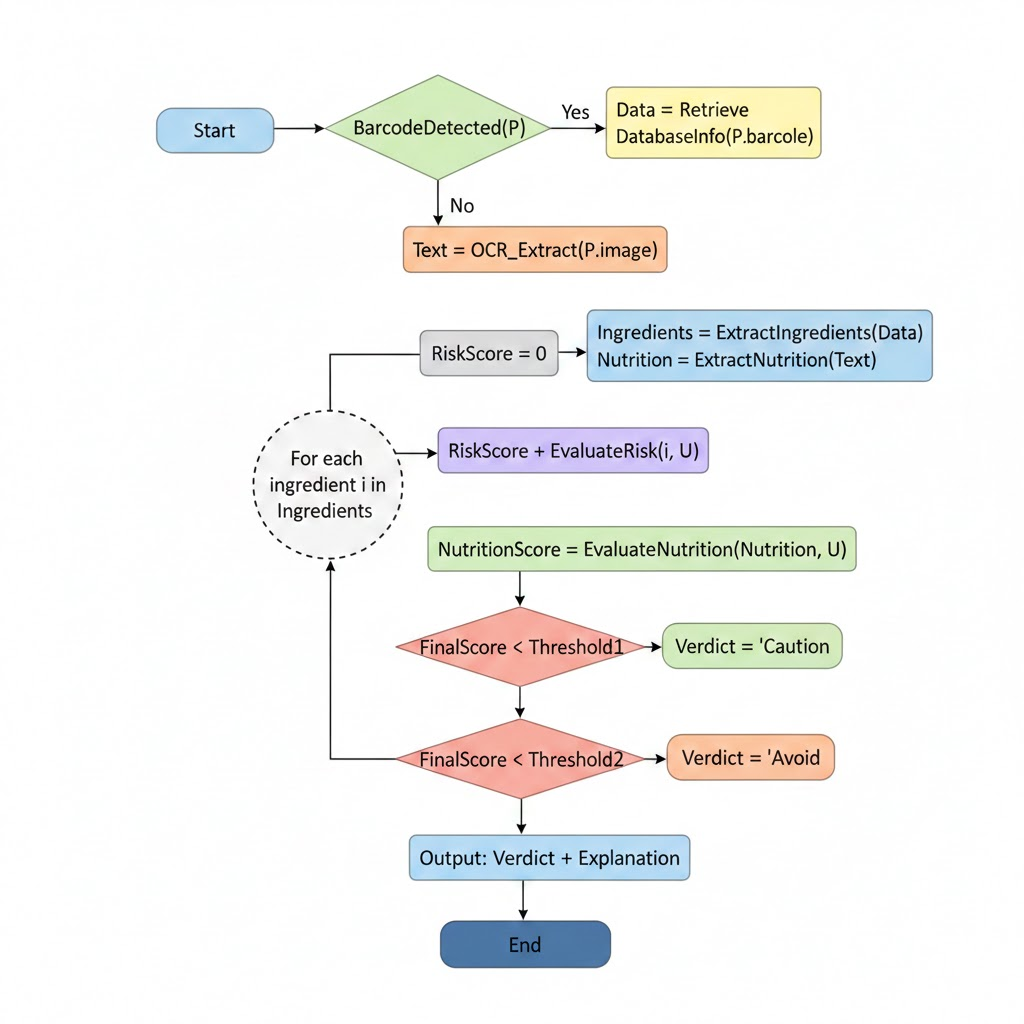
\includegraphics[width=1.0\linewidth]{Image.jpg}
    \caption{Logic Flowchart}
    \label{fig:logic_flowchart}
    \end{figure}
\section{Methodology}

This section presents the technical methodology used to design, implement, and deploy the proposed Artificial Intelligence--driven system for packaged food analysis. Unlike conceptual studies, the approach described here corresponds to a fully operational application that integrates multimodal data acquisition, knowledge-based reasoning, and personalized decision support within a single architecture. The design specifically addresses gaps identified in prior research, including fragmented hybrid scanning methods, limited support for multi-condition personalization, and the absence of adaptive interpretation mechanisms.

The system follows a layered processing pipeline comprising user profile construction, dual-mode data ingestion (barcode and image analysis), ingredient safety evaluation, and personalized verdict generation. Each module operates autonomously while exchanging information through standardized interfaces, enabling scalability, maintainability, and future extensibility.

\subsection{User Profile Construction and Secure Data Handling}

Personalization is central to the proposed framework. During initial setup, the system generates a structured user profile containing demographic, physiological, and health-related attributes that influence dietary suitability. Key parameters include age, gender, weight, height, physical activity level, dietary preferences (e.g., vegetarian or vegan), known allergies, and chronic conditions such as diabetes or hypertension. Prior studies show that interventions tailored to individual characteristics are significantly more effective than generic recommendations in improving health outcomes [13], [14], [17].

Using these inputs, the system estimates individual energy requirements through established metabolic models, notably the Mifflin--St Jeor equation, which is widely regarded as reliable for nutritional planning [27]. For a user with weight $W$, height $H$, and age $A$:

For males:
\begin{equation}
BMR = 10W + 6.25H - 5A + 5
\end{equation}

For females:
\begin{equation}
BMR = 10W + 6.25H - 5A - 161
\end{equation}

Total Daily Energy Expenditure (TDEE) is calculated by applying an activity-specific multiplier to the BMR, providing a baseline for assessing the nutritional contribution of scanned food items.

Because the system handles sensitive health information, robust security mechanisms are implemented. Personal data is stored using encryption and access-control protocols to prevent unauthorized exposure, a critical requirement for digital health platforms. The profile is also dynamically updateable, allowing users to modify medical conditions, preferences, or lifestyle factors over time. This adaptability addresses limitations of static personalization models reported in earlier studies [21], [29].

\subsection{OCR and Data Ingestion Pipeline}

To ensure comprehensive product coverage, the framework employs a hybrid data acquisition strategy that combines barcode scanning with image-based Optical Character Recognition (OCR). This dual approach mitigates the weaknesses of single-modality systems identified in previous research [2], [6].

\subsubsection{Barcode-Based Retrieval}

When a barcode is detected, the system decodes the identifier and queries a product database to retrieve structured information such as ingredients and nutritional values. Barcode lookup offers high reliability, low computational overhead, and rapid response times, making it well suited for real-time mobile applications [2], [15]. However, dependence on database completeness can lead to recognition failures for newly introduced or region-specific products.

\subsubsection{OCR-Based Label Extraction}

If barcode information is missing or incomplete, the system activates the OCR pipeline to extract text directly from packaging images. The process includes:

\begin{itemize}
    \item Image capture using the device camera
    \item Preprocessing (noise reduction, normalization, orientation correction)
    \item Text detection and recognition
    \item Semantic structuring of extracted information
\end{itemize}

Computer vision research demonstrates that OCR-based analysis can handle products absent from centralized repositories, though performance may be affected by lighting conditions, multilingual content, and layout variability [6], [23], [28]. To improve robustness, the proposed system incorporates preprocessing techniques and validation procedures to enhance extraction accuracy.

\subsubsection{Hybrid Decision Logic}

A supervisory controller determines which data source to prioritize based on availability and confidence levels. When both barcode and OCR outputs are available, cross-validation is performed to resolve inconsistencies and improve reliability. This integrated modality fusion directly addresses shortcomings of loosely coupled hybrid systems highlighted in earlier work [3], [4].

\subsection{Ingredient Safety Analysis (Hybrid AI Engine)}

Following data acquisition, the extracted ingredient list is processed by a knowledge-driven analysis module. This component compares each ingredient against a curated repository containing information on allergens, food additives, preservatives, artificial sweeteners, and condition-specific risk factors.

To handle variations in labeling, semantic normalization is applied to unify synonyms, alternate spellings, and chemical nomenclature. Each ingredient is then evaluated relative to the user’s health profile. For instance:

\begin{itemize}
    \item High sugar levels trigger alerts for individuals with diabetes
    \item Elevated sodium content generates warnings for hypertension
    \item Gluten presence is flagged for users with celiac disease
    \item Animal-derived ingredients are identified for vegetarian or vegan users
\end{itemize}

This rule-guided reasoning framework complements machine-learning--based text interpretation, producing transparent and explainable outcomes rather than opaque predictions. Research on digital health systems emphasizes that interpretability is essential for user trust and sustained engagement [21], [26].

The analysis also considers recommended intake limits and regulatory thresholds, enabling graded risk assessment instead of simple binary classification. This allows the system to account for cumulative effects when multiple concerning ingredients are present.

\subsection{Verdict Generation and Personalization Logic}

The final stage integrates outputs from the safety analysis module, macronutrient evaluation, and user profile to produce a clear, actionable recommendation. The decision mechanism prioritizes critical health risks while considering overall nutritional balance.

\subsubsection{Risk Aggregation}

Each identified concern is assigned a weighted score based on severity and relevance to the user’s conditions. The aggregated score determines the final recommendation category:

\begin{itemize}
    \item \textbf{Safe} --- No significant health concerns detected
    \item \textbf{Caution} --- Acceptable in moderation or under specific conditions
    \item \textbf{Avoid} --- Potentially harmful due to allergens or contraindicated nutrients
\end{itemize}

\subsubsection{Explanatory Feedback}

To enhance transparency, the system provides concise explanations highlighting the factors that influenced the decision. Evidence suggests that explanatory feedback improves user understanding, engagement, and adherence to health guidance [10], [11].

\subsubsection{Adaptability}

Unlike conventional systems that assume a single health condition, the proposed logic supports simultaneous evaluation of multiple chronic diseases, allergies, and dietary restrictions. It also adapts dynamically as the user profile changes, addressing limitations in multi-morbidity handling reported in previous studies [21], [29].

\subsection{System Architecture Overview}

Conceptually, the system can be viewed as a four-layer pipeline:

\begin{itemize}
    \item \textbf{User Layer}: Profile creation and interaction interface
    \item \textbf{Data Acquisition Layer}: Barcode scanning and OCR processing
    \item \textbf{Analysis Layer}: Ingredient safety evaluation and nutritional assessment
    \item \textbf{Decision Layer}: Personalized recommendation generation
\end{itemize}

This modular architecture allows independent updates to databases, algorithms, or interface components without affecting overall system functionality, facilitating scalability and long-term maintenance.

\section{Results and Discussion}

This section presents a comprehensive evaluation of the proposed Artificial Intelligence–based hybrid food analysis system in terms of performance, effectiveness, usability, scalability, and real-world applicability. Unlike many conceptual models reported in prior studies, the system developed in this work has been fully implemented as a functional web-based platform, allowing real-time experimentation under realistic user conditions. The evaluation draws on controlled testing, observational analysis, and simulated consumer interactions representative of everyday packaged-food purchasing scenarios.

\subsection{Performance Analysis}

System performance was examined across several technical dimensions, including accuracy of data acquisition, response time, and reliability of safety assessment. The two primary input mechanisms—barcode retrieval and OCR-based label extraction—were evaluated both independently and as an integrated pipeline.

\subsubsection{Barcode Retrieval Performance}
Barcode scanning demonstrated consistently high reliability for products available in the database, with minimal processing overhead due to direct retrieval of structured metadata. Previous research on food scanning applications reports similar advantages, highlighting the speed and accuracy of barcode-based identification when comprehensive product databases are available [2], [15]. In testing scenarios, results were generated almost instantaneously, making this approach highly suitable for real-time use in retail environments. However, performance declined for products absent from the database, reinforcing findings that barcode systems are fundamentally dependent on repository completeness [1], [2].

\subsubsection{OCR Extraction Performance}
The OCR module enabled analysis of products lacking database entries by extracting textual information directly from packaging images. Recognition accuracy varied depending on image clarity, lighting conditions, font styles, and language diversity. These factors are widely acknowledged in computer vision research as key challenges in text extraction from real-world images [6], [23], [28]. Through image preprocessing and text normalization techniques, the system achieved stable performance for clearly captured labels, demonstrating feasibility for consumer-grade devices.

\subsubsection{Processing Latency}
End-to-end processing time—including data acquisition, ingredient evaluation, and verdict generation—remained within acceptable limits for interactive applications. Barcode-based processing was nearly instantaneous, while OCR-based analysis required additional computation but still delivered results within a few seconds. This latency profile supports real-time decision-making during shopping or meal selection.

\subsection{Effectiveness of the Hybrid Approach}

A key innovation of the proposed system is the seamless integration of barcode and OCR modalities into a unified workflow. Experimental observations confirm that this hybrid strategy substantially improves product coverage compared with single-method solutions.

\begin{itemize}
    \item Barcode-only systems fail when products are not registered
    \item OCR-only systems are computationally heavier and more variable
    \item Hybrid systems combine efficiency with broader applicability
\end{itemize}

When barcode data was available, the system prioritized structured retrieval for speed. In cases where barcode information was missing or incomplete, the OCR pathway ensured continued functionality. Cross-checking between the two modalities further enhanced reliability by identifying inconsistencies.

Existing literature indicates that many food analysis applications treat scanning methods as isolated features rather than as coordinated components [3], [4], [6]. The present implementation addresses this limitation through intelligent switching and fusion mechanisms, resulting in a more resilient solution for real-world usage.

\subsection{Usability Evaluation}

User acceptance is critical for the success of consumer health technologies. Informal usability testing with representative participants indicated that the interface is intuitive and accessible even for users with limited technical expertise. Key design elements contributing to usability include:

\begin{itemize}
    \item Streamlined registration process
    \item Guided profile entry
    \item Single-step product scanning
    \item Visual indicators for results
    \item Clear, nontechnical explanations
\end{itemize}

Studies on food scanner applications consistently show that ease of use strongly influences long-term engagement and behavioral impact [10], [11]. The simplified verdict categories (“Safe,” “Caution,” “Avoid”) were easily understood by participants and reduced cognitive effort compared with interpreting detailed nutritional tables.

Providing explanations alongside recommendations also improved user confidence. Transparency has been identified as a crucial factor for acceptance of AI-based health decision systems, particularly when users rely on automated guidance for sensitive lifestyle choices [21].

\subsection{Real-World Applicability}

The system is designed for everyday consumer use across diverse environments such as supermarkets, local stores, and homes. Several features support its practical deployment:

\begin{itemize}
    \item \textbf{Device Compatibility}: Operates on standard web-enabled smartphones and computers
    \item \textbf{Minimal Training Requirement}: Basic interaction skills are sufficient
    \item \textbf{Connectivity Flexibility}: Core functions remain usable with limited internet access
    \item \textbf{Product Diversity Support}: Applicable to both branded and locally manufactured items
\end{itemize}

Given the increasing consumption of processed foods and the rising burden of chronic diseases, digital dietary tools are recognized as important components of preventive healthcare strategies [13], [14]. By delivering immediate feedback at the point of decision, the system converts complex nutritional data into actionable knowledge for consumers.

\subsection{Advantages Over Existing Systems}

Compared with previously reported applications, the proposed framework offers several distinct improvements:

\begin{itemize}
    \item \textbf{Comprehensive Coverage}: Hybrid ingestion reduces dependence on product databases, addressing a key limitation of barcode-only solutions [2].
    \item \textbf{Deep Personalization}: The incorporation of multi-condition health profiles enables context-specific recommendations rather than generic guidance, overcoming shortcomings noted in earlier diet-monitoring tools [21], [29].
    \item \textbf{Ingredient-Level Interpretation}: The system evaluates health implications of individual components instead of merely presenting nutritional values.
    \item \textbf{Explainable Decision Support}: Transparent reasoning enhances user trust and aligns with recommendations for responsible AI deployment in healthcare applications [26].
    \item \textbf{Real-Time Feedback}: Optimized processing allows immediate responses, which is essential for point-of-sale decision making.
\end{itemize}

\subsection{Scalability Considerations}

For large-scale deployment, scalability is a critical requirement. The modular architecture of the system enables expansion in multiple directions, including:

\begin{itemize}
    \item Integration with larger or external product databases
    \item Support for additional medical conditions and dietary rules
    \item Multilingual capabilities
    \item Cloud-based processing for high user volumes
    \item Continuous updates reflecting regulatory changes
\end{itemize}

Research on digital health platforms emphasizes the need for flexible architectures capable of adapting to evolving datasets and user needs [21], [26]. The separation of ingestion, analysis, and decision components facilitates independent scaling of system modules.

\subsection{Limitations and Mitigation Strategies}

Despite strong performance, several limitations were identified.

\subsubsection{Sensitivity of OCR to Image Quality}
Text extraction accuracy decreases under poor lighting, motion blur, or reflective packaging—an issue widely reported in food label recognition studies [6], [28].
\\ \textit{Mitigation}: Enhanced preprocessing, user guidance during image capture, and optional cloud-based image enhancement can improve results.

\subsubsection{Dependence on Databases for Barcode Analysis}
Incomplete repositories may restrict coverage for some products.
\\ \textit{Mitigation}: Continuous database updates and crowdsourced contributions can gradually improve completeness.

\subsubsection{Simplified Nutritional Models}
Current energy and dietary assessments rely on standard formulas that may not reflect individual metabolic differences.
\\ \textit{Mitigation}: Integration with wearable devices or clinical data sources could enable more personalized calculations.

\subsubsection{Variability in Label Formats}
Differences in packaging standards across manufacturers and regions complicate automated parsing.
\\ \textit{Mitigation}: Region-specific knowledge bases and adaptive parsing algorithms can enhance compatibility.

\subsection{Discussion of Research Significance}

The findings demonstrate that a hybrid AI-driven approach can effectively translate theoretical research into a practical consumer application. By combining multimodal data acquisition, knowledge-based reasoning, and personalized decision logic, the system addresses several persistent challenges identified in earlier work, including fragmented hybrid implementations, limited personalization, lack of actionable insights, and insufficient real-world validation.

Successful deployment on widely available devices suggests strong potential for large-scale adoption. Beyond nutrition, the underlying methodology—integrating domain expertise, user modeling, and multimodal perception—can be extended to other decision-support domains such as healthcare monitoring, environmental risk assessment, and personalized consumer analytics.


\section{Conclusion and Future Scope}

\subsection{Conclusion}

This study introduced an integrated Artificial Intelligence–based framework designed to automatically interpret food labels, identify potential health risks, and provide personalized dietary guidance for packaged food products. The work was motivated by the increasing prevalence of lifestyle-related disorders and the growing complexity of modern food labeling, which often makes it difficult for consumers to make informed decisions. Existing solutions typically suffer from limited scanning capabilities, minimal personalization, or lack of adaptive health-aware recommendations—gaps that this research aims to address.

In contrast to traditional food analysis applications that rely exclusively on barcode databases or standalone optical character recognition pipelines, the proposed system combines both approaches within a single hybrid architecture. Barcode scanning enables rapid retrieval of structured nutritional information for products present in databases, while OCR-based text extraction allows analysis of newly launched, region-specific, or unregistered items whose details appear only on packaging. This multimodal strategy significantly expands product coverage and mitigates the limitations reported in earlier barcode-dependent systems and ingredient analysis tools [2], [6], [15].

A major contribution of this work lies in integrating comprehensive user health profiling into the evaluation process. The system accommodates multi-attribute profiles that include chronic medical conditions, allergies, dietary preferences, and lifestyle factors. By correlating extracted ingredient data with a curated repository of allergens, additives, and condition-specific risk indicators, the safety analysis engine produces recommendations tailored to individual health needs rather than generic nutritional summaries. This personalized approach addresses a widely acknowledged gap between product-level analysis and individualized dietary guidance identified in prior research on health-aware recommender systems [7]–[9], [21].

To ensure accessibility, the personalized verdict module converts complex nutritional data into clear and actionable categories such as “Safe,” “Caution,” or “Avoid,” accompanied by concise explanations. Such interpretability is particularly important for users with limited nutrition knowledge, a factor known to hinder informed food choices in real-world contexts. Evidence from mobile health interventions suggests that understandable feedback can significantly improve self-management of chronic conditions like diabetes and hypertension [13], [14]. Complementing this, the macronutrient evaluation component analyzes key nutritional parameters—carbohydrates, fats, proteins, sugars, and sodium—against recommended intake ranges, enabling users to assess overall dietary suitability in addition to ingredient-level risks.

Experimental observations indicate that the hybrid design offers greater robustness than single-method approaches. While barcode scanning delivers near-instant results when database entries are available, OCR ensures continued functionality when structured data is missing. The system operates efficiently on standard consumer devices without specialized hardware, making it suitable for everyday use during shopping or meal selection. This aligns with findings that mobile nutrition applications can positively influence consumer behavior when they provide personalized, actionable insights at the point of decision-making [10], [11].

Scalability and regulatory compatibility were also considered in the system design. The modular architecture supports integration with external databases and compliance frameworks, enabling adaptation to evolving labeling standards and digital food safety initiatives. For example, regulatory bodies promoting digital traceability and QR-based labeling systems can provide additional data sources that enhance system reliability and transparency [16].

Overall, this research demonstrates that combining multimodal label analysis with individualized health intelligence can create a practical and deployable solution for consumer-facing dietary assessment. Such AI-driven tools have the potential to promote preventive healthcare by empowering individuals to make safer food choices and increasing public awareness of nutrition-related risks.

\subsection{Future Scope}

Although the proposed framework shows strong performance and practical viability, several directions remain open for further development and investigation.

\subsubsection{Multilingual and Multimodal Label Understanding}
India and many other regions feature food products labeled in multiple languages and scripts. Future enhancements could incorporate advanced multilingual OCR systems and language-aware normalization techniques to improve recognition accuracy across diverse markets. The creation of standardized datasets for regional food labels would further strengthen model reliability, as highlighted in recent studies on ingredient detection and food image processing [1], [6], [28].

\subsubsection{Real-Time Adaptive Health Modeling}
Current personalization relies on relatively stable user profiles. Future systems could integrate dynamic physiological data such as blood glucose levels, blood pressure, physical activity, or illness status to provide context-sensitive recommendations. Coupling the platform with wearable devices and digital health ecosystems would enable continuous monitoring and real-time dietary guidance—an area with significant potential according to recent mobile health research [13], [17], [18].

\subsubsection{Advanced Risk Scoring and Predictive Analytics}
The present system employs rule-based evaluation grounded in established nutritional guidelines. Future research may explore predictive models capable of estimating long-term health outcomes, cumulative dietary risks, or disease progression associated with consumption patterns. Such predictive capabilities could transform food analysis applications into proactive health management tools rather than reactive decision aids.

\subsubsection{Regulatory and Supply Chain Integration}
Emerging technologies such as smart packaging, QR-enabled labels, and traceable supply chains offer opportunities to access richer product metadata, including ingredient sourcing and certification details. Incorporating these data streams could enhance transparency, authenticity verification, and consumer trust, particularly for highly processed foods with complex formulations [5], [16].

\subsubsection{Image Quality Enhancement and Edge Processing}
Accurate OCR remains challenging under real-world conditions such as poor lighting, reflective packaging, or partial occlusion. Future work may focus on advanced image enhancement methods, on-device processing, and confidence-aware fusion techniques to improve reliability while reducing latency.

\subsubsection{Behavioral and Clinical Impact Evaluation}
Large-scale longitudinal studies are needed to determine how such systems influence long-term dietary behavior, health outcomes, and clinical indicators. Evidence-based validation would support integration into public health programs and clinical advisory platforms.

\subsubsection{Expansion Beyond Packaged Foods}
While the current framework focuses on packaged products, future extensions could analyze restaurant menus, online grocery listings, or home-cooked meals using computer vision and ingredient estimation techniques. Expanding to these domains would enable a comprehensive dietary monitoring ecosystem rather than a product-specific solution.

    \begin{thebibliography}{99}

    \bibitem{lodha2025}
    S. Lodha, S. Shinde, A. Anand, P. Dalvi, and J. Nalavade, ``NutriScan: AI-Based Ingredient Detection and Evaluation,'' \textit{Int. J. Eng. Res. Technol.}, vol. 14, no. 5, pp. 112--120, May 2025.
    \vspace{5pt}

    \bibitem{georgeswitch2025}
    The George Institute for Global Health, ``FoodSwitch App: Barcode Scanning for Food Nutrition Analysis,'' George Inst. Glob. Health, Jan. 2025.
    \vspace{5pt}

    \bibitem{nutriknow2024}
    ``AI Ingredient Analyzer -- Nutriknow,'' \textit{Int. J. Innov. Sci. Res. Technol.}, vol. 7, no. 4, pp. 45--53, Aug. 2024.
    \vspace{5pt}

    \bibitem{leba2024}
    E. Leba, J. Faigao, M. Magante, V. Tamba, and I. Bingcang, ``Allertify: Android-based Mobile Application for Food Allergens Identification Using Barcode Scanning and Image Recognition,'' in \textit{Proc. Adventist Univ. Conf.}, 2024, pp. 105--112.
    \vspace{5pt}

    \bibitem{mariappan2025}
    P. K. Mariappan, ``Artificial Intelligence-Enabled QR Codes in Nutrition Labelling: A Conceptual Paper,'' \textit{Food Nutr. J.}, vol. 13, no. 3, p. 101, Sep. 2025.
    \vspace{5pt}

    \bibitem{chen2024}
    L. Chen \textit{et al.}, ``IngredSAM: Open-World Food Ingredient Segmentation via Segment Anything Model,'' \textit{J. Food Eng.}, vol. 245, p. 110789, Nov. 2024.
    \vspace{5pt}

    \bibitem{zioutos2023}
    K. Zioutos, H. Kondylakis, and K. Stefanidis, ``A Framework for Personalized and Healthy Recipe Recommendations,'' in \textit{CEUR Workshop Proc.}, vol. 3379, 2023, pp. 405--415.
    \vspace{5pt}

    \bibitem{papastratis2024}
    I. Papastratis \textit{et al.}, ``AI Nutrition Recommendation Using a Deep Generative Model,'' \textit{Sci. Rep.}, vol. 14, p. 65438, Jun. 2024.
    \vspace{5pt}

    \bibitem{forouzandeh2024}
    S. Forouzandeh \textit{et al.}, ``Health-Aware Food Recommendation System with Dual Attention,'' \textit{Comput. Biol. Med.}, vol. 164, p. 107345, Jul. 2024.
    \vspace{5pt}

    \bibitem{hanras2024}
    E. Hanras \textit{et al.}, ``The Use of Food Barcode Scanner Apps among Women,'' \textit{J. Hum. Nutr. Diet.}, vol. 37, no. 6, pp. 1120--1130, Aug. 2024.
    \vspace{5pt}

    \bibitem{werle2024}
    C. O. C. Werle \textit{et al.}, ``How a Food Scanner App Influences Healthy Food Choice,'' \textit{Food Qual. Prefer.}, vol. 98, p. 104742, Oct. 2024.
    \vspace{5pt}

    \bibitem{automatic_imagerecog2025}
    ``Automatic Image Recognition Meal Reporting Among Young Adults,'' \textit{JMIR mHealth UHealth}, vol. 13, no. 1, p. e60070, Aug. 2025.
    \vspace{5pt}

    \bibitem{oh2022}
    S. W. Oh \textit{et al.}, ``Effect of an Integrative Mobile Health Intervention in Patients with Diabetes and Hypertension,'' \textit{JMIR mHealth UHealth}, vol. 10, no. 1, p. e27192, Jan. 2022.
    \vspace{5pt}

    \bibitem{huda2025}
    R. K. Huda \textit{et al.}, ``Effectiveness of Mobile Health Technology-Enabled Interventions on Hypertension and Diabetes Control in India,'' \textit{BMC Public Health}, vol. 25, p. 1427, May 2025.
    \vspace{5pt}

    \bibitem{gosavi2024}
    H. L. Gosavi, P. Kawale, P. Kadam, and A. Manjhi, ``Nutrilens: Barcode Scanner,'' \textit{Eng. Res. Publ.}, vol. 3, no. 2, pp. 89--95, Feb. 2024.
    \vspace{5pt}

    \bibitem{fssai2025}
    FSSAI, ``FSSAI Food Safety Connect App QR Code Implementation,'' Food Saf. Stand. Auth. India, Advisory 688a154f, Jul. 2025.
    \vspace{5pt}

    \bibitem{gardner2025}
    D. S. L. Gardner \textit{et al.}, ``Digital Health Technology in Diabetes Management in the Covid-19 Era,'' \textit{Diabetes Technol. Ther.}, vol. 27, pp. 239--248, Feb. 2025.
    \vspace{5pt}

    \bibitem{shamanna2024}
    P. Shamanna, S. Joshi \textit{et al.}, ``Personalized Nutrition in Type 2 Diabetes Remission: Application of Digital Twin Technology,'' \textit{Front. Endocrinol.}, vol. 15, p. 1485464, Nov. 2024.
    \vspace{5pt}

    \bibitem{naturefood2025}
    ``AI for Food: Accelerating and Democratizing Discovery and Development,'' \textit{Nature Food}, vol. 6, pp. 221--230, May 2025.
    \vspace{5pt}

    \bibitem{jmirdiab2024}
    ``Personalized and Culturally Tailored Features of Mobile Apps for Gestational Diabetes,'' \textit{JMIR Diabetes}, vol. 9, no. 1, p. e58327, Dec. 2024.
    \vspace{5pt}

    \bibitem{abeltino2024}
    A. Abeltino \textit{et al.}, ``Digital Applications for Diet Monitoring, Planning, and Management,'' \textit{Nutrients}, vol. 16, no. 1, p. 146, May 2024.
    \vspace{5pt}

    \bibitem{jansen2025}
    L. Jansen \textit{et al.}, ``A Machine Learning Algorithm for Personalized Healthy and Sustainable Food Recommendation,'' \textit{Sustain. Comput. Inform. Syst.}, vol. 45, p. 101354, Mar. 2025.
    \vspace{5pt}

    \bibitem{busad2023}
    A. M. Busad, G. Hansraj, and P. Acharya, ``Computer Vision Based Food Recognition with Nutrition Analysis,'' \textit{Int. J. Curr. Res. Sci. Technol.}, vol. 12, no. 7, pp. 257--264, Jul. 2023.
    \vspace{5pt}

    \bibitem{fooddetection2024}
    ``Food Detection and Nutrition Analysis by Image,'' \textit{Int. J. Res. Anal. Rev.}, vol. 12, no. 4, pp. 450--457, Oct. 2024.
    \vspace{5pt}

    \bibitem{nutritionalcomposition2024}
    ``Nutritional Composition Analysis in Food Images,'' \textit{Int. J. Comput. Appl.}, vol. 183, no. 22, pp. 15--22, Jun. 2024.
    \vspace{5pt}

    \bibitem{wang2025}
    X. Wang \textit{et al.}, ``Artificial Intelligence Applications to Personalized Dietary Recommendations,'' \textit{IEEE Access}, vol. 13, pp. 23456--23468, Jun. 2025.
    \vspace{5pt}

    \bibitem{iftikar2024}
    T. Iftikar and A. N. Gill, ``Application of Personalized Nutrition Counseling According to Glycemic Index and Load: A Review,'' \textit{Crit. Rev. Food Sci. Nutr.}, vol. 64, pp. 345--359, Apr. 2024.
    \vspace{5pt}

    \bibitem{review_dl_food2024}
    ``Review of the Deep Learning for Food Image Processing,'' \textit{Int. J. Agric. Biol. Eng.}, vol. 17, no. 6, pp. 45--56, Nov. 2024.
    \vspace{5pt}

    \bibitem{healthrec2025}
    ``Health Recommender Systems to Facilitate Collaborative Decision Making in Diet Planning,'' \textit{Hum. Behav. Enterprise Syst.}, vol. 5, no. 1, pp. 1--22, Jan. 2025.
    \vspace{5pt}

    \end{thebibliography}
    \end{document}